\section{Introduction}
\label{sec:intro}

% General motivation
The importance of networks in scientific and commercial domains cannot
be overstated.  
Considerable research and engineering effort is being devoted to developing
effective and efficient graph representations and analytics.
Efficient graph abstractions and analytics for {\em static graphs} are
to researchers and practitioners in scope of open source platforms
such as Apache Giraph, Apache Spark (through
GraphX~\cite{DBLP:conf/osdi/GonzalezXDCFS14} and GraphLab (through
the PowerGraph library~\cite{DBLP:conf/osdi/GonzalezLGBG12}).
\eat{ This in
  turn makes sophisticated graph analysis methods available to
  researchers and practitioners, facilitating their widespread
  adoption. Further, because these systems are open source, this
  encourages development and dissemination of new graph analysis
  methods, and of more efficient implementations of existing methods.}

%Arguably the most interesting and important questions one can ask
%about networks have to do with their evolution, rather than with their
%static state.  
Analysis of {\em evolving graphs} has been receiving
increasing attention~\cite{DBLP:journals/csur/AggarwalS14,Chan2008,Kan2009,DBLP:journals/tos/MiaoHLWYZPCC15,Ren2011,Semertzidis2015}.
%Some areas where evolving graphs are being studied are social network
%analysis,
%biological networks and the Web.
%\eat{~\cite{DBLP:conf/icwsm/GoetzLMF09,DBLP:journals/tweb/LeskovecAH07,DBLP:conf/kdd/LeskovecBKT08,DBLP:conf/icml/SarkarCJ12}},
%biological networks~\cite{DBLP:journals/tkdd/AsurPU09,DBLP:journals/tcsb/BeyerTLSF10,Stuart2003} and the Web~\cite{DBLP:journals/kais/ChanBL08,DBLP:journals/jisa/PapadimitriouDG10}.
%
Yet, despite the recent activity, and
despite increased variety and availability of evolving graph data,
{\em systematic support for scalable querying and analytics over
  evolving graphs still lacks}.  This support is urgently needed, due
first and foremost to the scalability and efficiency challenges
inherent in evolving graph analysis, but also to considerations of
usability and ease of dissemination.  {\em In this paper, we present
  \ql, a system for scalable exploratory analysis of evolving graphs,
  that fills this gap.}

\ql represents the evolution of a graph, including changes in topology 
or attribute values of vertices and edges, continuously through time
using the \tg abstraction.  An example of a \tg is given in
Figures~\ref{fig:tg_rg} and~\ref{fig:tg_ve}.  Figure~\ref{fig:tg_rg} gives the
{\em representative graphs} of a \tg --- a sequence of
graphs associated with a sequence of coalesced time periods.  The semantics
is that no change occurred in a graph for the duration of
the time period. Figure~\ref{fig:tg_ve} gives the {\em vertex-edge}
representation of an evolving graph --- a collection of coalesced
temporal SQL relations with appropriate integrity constraints.
The \ql system implements the \tg abstraction and the operations of a
fully compositional algebra, supporting exploratory analysis. 
Consider these questions over evolving graphs:

\eat{Quick overview of our model and operations.  Point to a
  figure.  We represent graph evolution through a continuous time
  period, graphs have attributes on vertices and edges, vertex and
  edge schemas may evolve.  For graph analysis, it is often useful to
  compute representative graphs - an aggregated view of an evolving
  graph by change or by time period, with quantification.
  Corroborating / complementing information from different sources -
  graph union and intersection.  Graph analytics.}
%

{\em Which network nodes are showing an increasing (decreasing) popularity trend,
  or have increasing influence?}
Node popularity can be quantified by, e.g., node degree, centrality measures,
or PageRank score.  This information can be used to prioritize
crawling on the Web, to target ads in a social network, and to
captures the dynamics of zeitgeist in semantic knowledge bases.
%
{\em Have any changes in network connectivity been observed, either
  suddenly or gradually?} Connectivity can be quantified as,
e.g., pair-wise distance, length of shortest path between communities,
or graph density.  For networks describing insulin-based metabolism
pathways, gradual pathway disruption can be used to determine the
onset of type-2 diabetes~\cite{DBLP:journals/tcsb/BeyerTLSF10}.  For a
website accessibility network, sudden loss of connectivity can signal
that censorship is taking place.\eat{ In a co-authorship network,
increasing connectivity among topical communities indicates stronger
collaboration across domains.}
%
\ql supports efficient computation of node popularity and network
connectivity measures with a combination of {\em temporal aggregation}
and {\em temporal analytics}.

{\em At what time scale can interesting trends be observed?} The
answer to this question may not be known a priori, at the time when
graph evolution data is being recorded.  Changes in node centrality in
a social network may be observable on the scale of weeks, but not
months.  On the Web, periodic events may change popularity
of websites, with observable trends on the scale of days, but not
hours or months.  Furthermore, the same network may
exhibit different trends at different time scales, e.g., node
popularity may change at a different rate than over-all network
density.  \ql supports this analysis via {\em temporal aggregation}.

{\em Can information about graph evolution be used to make graph
  analytics more stable?}  Algorithms that compute
website popularly can be vulnerable to link spam, but the identity 
of spammers is transient~\cite{DBLP:conf/cikm/YangQZGL07}.  Persistence 
vs. transience of a node, edge, or, more 
generally, of a subgraph, is a meaningful aspect of quality.  
\eat{Stable 
or representative subgraphs have also been used to improve performance 
of iterative computations in evolving graphs, e.g., for computing shortest
paths~\cite{Ren2011}.
}  The {\em temporal aggregation} operation in \ql
\eat{, available in several interesting variants, }can be used to find
representative subgraphs of an evolving graph.

{\em How can multiple data sources be used jointly to complement or
  corroborate information about graph evolution?}  \eat{It may be the
  case that m}Multiple datasets may be available, each describing a
series of crawls of different but possibly overlapping portions of
the Web graph.  Further, network states may be recorded at different,
possibly overlapping, time periods, or at different temporal scales.
Can these datasets be unified to support
analysis \eat{or meta-analysis }of network evolution trends?  \ql
supports {\em union} and {\em intersection} operations over evolving
graphs that enable this analysis.

\begin{figure}[t!]
%\centering
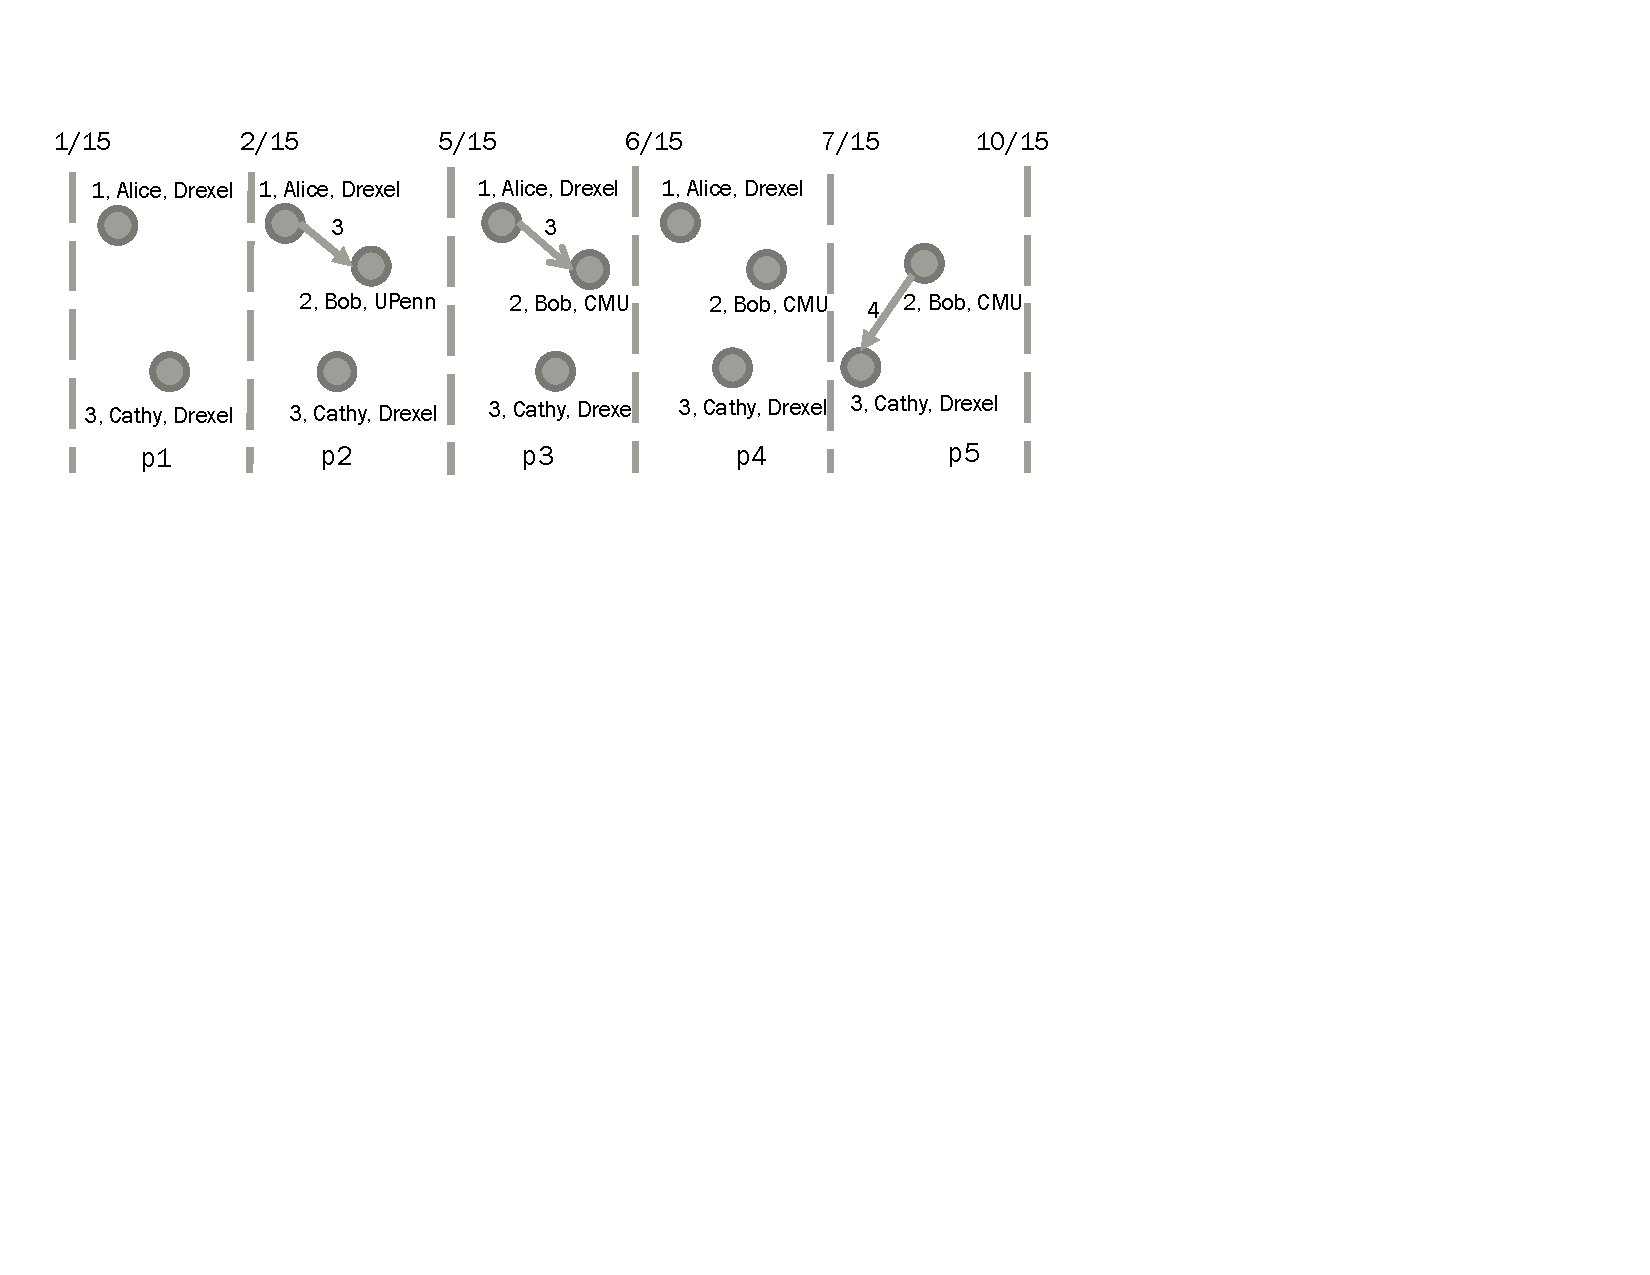
\includegraphics[width=3.4in]{figs/T1_graphs.pdf}
\vspace{-0.5cm}
\caption{Representative graphs of \tg \insql{T1}.}
\vspace{-0.4cm}
\label{fig:tg_rg}
\end{figure}

{\bf Contributions.} We make the following contributions to support
efficient and usable analysis of evolving graphs.

\begin{enumerate}[noitemsep,leftmargin=*]
%\begin{description}[noitemsep]

\item We propose a novel representation of an evolving graph, called a \tg,
  which captures the evolution of both graph topology and vertex and edge attributes (Section~\ref{sec:model}).  

\item We define a fully compositional \tg algebra, which includes
  temporal selection, subgraph, map, aggregation, join, union, and a
  rich class of analytics (Section~\ref{sec:algebra}).

\item We develop several physical representations of the logical \tg
  data structure corresponding to different trade-offs in temporal and
  structural locality, and implement these \eat{physical
  }representations and the operations of \tg algebra in Apache Spark,
  leveraging the GraphX
  framework~\cite{DBLP:conf/osdi/GonzalezXDCFS14} 
  (Section~\ref{sec:sys}).  \eat{
\item We support efficient execution of
  Pregel-style~\cite{DBLP:conf/sigmod/MalewiczABDHLC10} analytics over the
  representative graphs of a \tg.  We also support efficient
  computation of trends over attribute values, which may themselves be
  computed, e.g., by applying a graph analytic in the previous step.
  Our support of graph analytics is discussed in
  Section~\ref{sec:analytics}.}

\item We conduct an extensive experimental evaluation with real
  datasets, demonstrating that \ql scales
  (Section~\ref{sec:exp}).\eat{, and also briefly discuss the
    usability of our framework in this section}

%\end{description}
\end{enumerate}

\eat{Our language supports a variety of operations including temporal
selection, join, and aggregation, and a rich class of analytics.
Further, we provide a scalable and extensible open-source
implementation of \ql in scope of Apache Spark, an open-source
distributed data processing framework.  We develop several novel
physical representations of evolving graphs, and novel partitioning
strategies that explore the trade-off between structural and temporal
locality.  We experimentally demonstrate that good performance can be
achieved with careful engineering.}

\eat{ {\bf Roadmap.}  We present our model in Section~\ref{sec:model}.
  We describe the \ql query language in Section~\ref{sec:example}, and
  discuss its implementation in an open-source prototype in
  Section~\ref{sec:sys}.  Section~\ref{sec:exp} describes our
  extensive experimental evaluation on real datasets.  We discuss
  related work in Section~\ref{sec:related}.  Future work and
  conclusions are given in Section~\ref{sec:conc}.}
